\documentclass{article}
\usepackage{tikz}
\usepackage[utf8]{inputenc}
\usetikzlibrary{arrows,automata}
\usepackage[all]{xy}
\usepackage{enumerate}
\usepackage{amsfonts}
\usepackage{qtree}


\title{Práctica 5: Gramáticas libres de contexto}
\author{Lothar Soto Palma DNI:49079173W}
\date{\today}

\begin{document}

\maketitle

\section*{Ejercicio 1:}
Demuestra que la siguiente gramática libre de contexto es ambigua.\\ 
\begin{center}
 \begin{tabular}{l|l}
$S\rightarrow S_1S_2$ & $S\rightarrow S_4S_5$ \\ 
$S_1\rightarrow aS_1b|\varepsilon$ & $S_4\rightarrow aS_4|S_6$ \\
$S_2\rightarrow cS_2|S_3$ &  $S_6\rightarrow bS_6|\varepsilon$\\
$S_3\rightarrow dS_3|\varepsilon$ &  $S_5\rightarrow cS_5d|\varepsilon$\\
\end{tabular}
 \end{center} 
\begin{itemize}
	\item Determina el lenguaje que genera esta gramática.
	\item Encuentra una gramática no ambigua que genere el lenguaje. 
\end{itemize}

Solución:
Podemos comprobar que la gramática es ambigua puesto que podemos formar dos arboles distintos para una misma palabra por ejemplo si tomamos la palabra $abcd$:\\\\
\Tree [.S [.$S_1$ a [.$S_1$ $\varepsilon$ ] b ] [.$S_2$ c [.$S_2$ [.$S_3$ d [.$S_3$ $\varepsilon$ ] ] ] ] ]
\Tree [.S [.$S_4$ a [.$S_4$ [.$S_6$ b [.$S_6$ $\varepsilon$ ] ] ] ] [.$S_5$ c [.$S_5$ $\varepsilon$ ] d ] ]

\begin{itemize}
	\item El lenguaje que genera esta gramática es la unión de los lenguajes $L_1, L_2$ que se definen de la siguiente forma:\\
$$L_1 = \{ a^ib^ic^jd^k : i,j,k \geq 0\}, 
L_2 = \{ a^ib^jc^kd^k : i,j,k \geq 0\}$$
$$L = L_1\cup L_2 = \{ a^ib^ic^jd^k : i,j,k \geq 0\}\cup \{ a^ib^jc^kd^k : i,j,k \geq 0\}$$
	\item Una gramática no regular es la siguiente:\\\\
	\begin{tabular}{l|l|l}
	$S\rightarrow S_1S_2$ & $S\rightarrow S_5S_6$ & $S\rightarrow S_9S_{10}$ \\
	$S_1\rightarrow aS_1b | \varepsilon$ & $S_5\rightarrow aS_5b | S_7 | S_8$ & $S_9\rightarrow aS_9b | \varepsilon$ \\
	$S_2\rightarrow cS_2d | S_3 | S_4$ & $S_6\rightarrow cS_6d|\varepsilon$ & $S_{10}\rightarrow cS_{10}d | \varepsilon$\\
	$S_3\rightarrow cS_3 | c$ & $S_7\rightarrow aS_7 | a$ & \\ 
	$S_4\rightarrow dS_4 | d$ & $S_8\rightarrow bS_8 | b$ & \\
	\end{tabular} 
\end{itemize}

\section*{Ejercicio 2:}
Dada la gramática:
$$S\rightarrow 01S, S\rightarrow 010S, S\rightarrow 101S, S\rightarrow  \varepsilon$$
\begin{itemize}
	\item Determina si es ambigua.
	\item ¿Eres capaz de encontrar una gramática regular que genere este lenguaje y que sea no ambigua?.
\end{itemize}

Solución:
\begin{itemize}
	\item La gramática es ambigua puesto que podemos representar la palabra $01010101$:\\\\
	\Tree [.S 0 1 [.S 0 1 [.S 0 1 [.S 0 1 [.S $\varepsilon$ ] ] ] ] ]\\
	\Tree [.S 0 1 [.S 0 1 0 [.S 1 0 1 [.S $\varepsilon$ ] ] ] ]
	\item Representamos la gramática ambigua como el siguiente autómata  finito no determinista:
	 \begin{center}
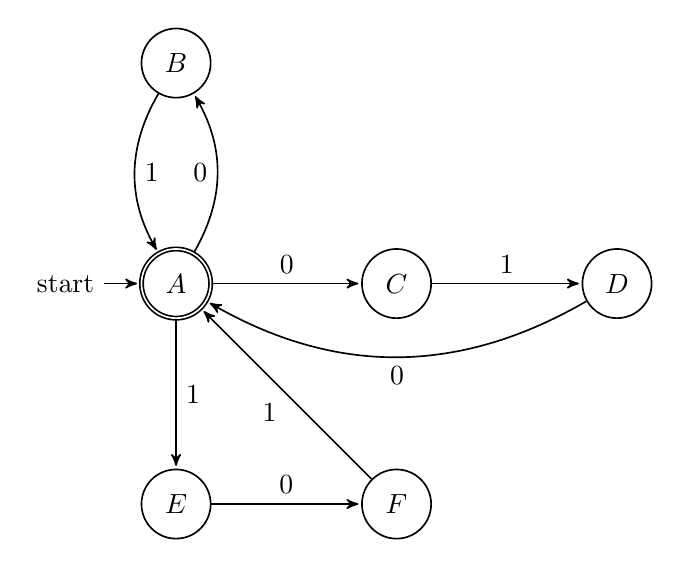
\begin{tikzpicture}[->,>=stealth',shorten >=1pt,auto,node distance=2.8cm,semithick]

	\node[state,initial,accepting]	(A)	{$A$};
	\node[state]	(B)	[above of=A] {$B$};
	\node[state] [right of=A] (C)	{$C$};
	\node[state] [right of=C] (D)	{$D$};
	\node[state] [below of=A] (E)	{$E$};
	\node[state] [right of=E] (F)	{$F$};

	\path (A) edge node {$0$} (C)
		(A) edge [bend right] node {$0$} (B)
		(B) edge [bend right] node {$1$} (A)
		(C) edge node {$1$} (D)
		(D) edge [bend left] node {$0$} (A)
		(A) edge node {$1$} (E)
		(E) edge node {$0$} (F)
		(F) edge node {$1$} (A);

\end{tikzpicture}
\end{center}
Convertimos el autómata en uno finito determinista y obtenemos la siguiente gramática:
$$S\rightarrow 0S_1 | 1S_2 | \varepsilon$$
$$S_1 \rightarrow 1S_3$$
$$S_2\rightarrow 0S_7$$
$$S_3\rightarrow 0S_4 | 1S_2 | \varepsilon$$
$$S_4\rightarrow 0S_1 | 1S_5 | \varepsilon$$ 
$$S_5\rightarrow 0S_6 | 1S_2 | \varepsilon $$
$$S_6\rightarrow 0S_1 | 1S_5 | \varepsilon$$
$$S_7\rightarrow 1S$$
\end{itemize}

\section*{Ejercicio 3:}
Pasa a Forma Normal de Chomsky la siguiente gramática libre de contexto:\\\\
$$S\rightarrow S_1 | S_2S_3a | aS_4cd | S_5S_4S_6$$
$$S_1 \rightarrow aS_1b | c$$
$$S_2\rightarrow S_3S_4 | S_5S_3d | S_1d | \varepsilon$$
$$S_3\rightarrow S_3c | S_2b | S_1aS_5 | c$$
$$S_4\rightarrow aS_4d | S_4d|\varepsilon$$
$$S_5\rightarrow aaS_5S_2 | S_5S_6S_7$$ 
$$S_6\rightarrow aS_6d | d$$
En primer lugar buscamos las producciones inutiles, para ello buscamos las producciones con simbolos terminales. Declaramos la variable $V_t$ entonces:
$$V_t=\{\emptyset\}, V_t=\{S_1,S_2,S_3,S_4,S_6\}, V_t=\{S,S_1,S_2,S_3,S_4,S_6\}$$
Eliminamos las producciones de $S_5$:
$$S\rightarrow S_1 | S_2S_3a | aS_4cd$$
$$S_1 \rightarrow aS_1b | c$$
$$S_2\rightarrow S_3S_4 | S_1d | \varepsilon$$
$$S_3\rightarrow S_3c | S_2b | c$$
$$S_4\rightarrow aS_4d | S_4d|\varepsilon$$ 
$$S_6\rightarrow aS_6d | d$$
Ahora eliminamos los estados con simbolos inaccesibles:
$$J=\{S\}, V_s=\{S\}, T_s=\{\emptyset\}$$
$$J=\{S_1,S_2,S_3,S_4\}, V_s=\{S,S_1,S_2,S_3,S_4\}, T_s=\{a,c,d\}$$
$$J=\{S_2,S_3,S_4\}, V_s=\{S,S_1,S_2,S_3,S_4\}, T_s=\{a,b,c,d\}$$
$$J=\{S_3,S_4\}, V_s=\{S,S_1,S_2,S_3,S_4\}, T_s=\{a,b,c,d,\varepsilon\}$$
$$J=\{S_4\}, V_s=\{S,S_1,S_2,S_3,S_4\}, T_s=\{a,b,c,d,\varepsilon\}$$
$$J=\{\emptyset\}, V_s=\{S,S_1,S_2,S_3,S_4\}, T_s=\{a,b,c,d,\varepsilon\}$$
Por lo que podemos eliminar la producción $S_6$:
$$S\rightarrow S_1 | S_2S_3a | aS_4cd$$
$$S_1 \rightarrow aS_1b | c$$
$$S_2\rightarrow S_3S_4 | S_1d | \varepsilon$$
$$S_3\rightarrow S_3c | S_2b | c$$
$$S_4\rightarrow aS_4d | S_4d|\varepsilon$$ 
Ahora eliminamos las producciones nulas:
$$H=\{\emptyset\}, H=\{S_2S_4\}, H=\{S_2S_4\}$$
Por lo que obtenemos:
$$S\rightarrow S_1 | S_2S_3a | S_3a | aS_4cd | acd$$
$$S_1 \rightarrow aS_1b | c$$
$$S_2\rightarrow S_3S_4 | S_3 | S_1d$$
$$S_3\rightarrow S_3c | S_2b | b | c$$
$$S_4\rightarrow aS_4d | ad |S_4d | d$$ 
Ahora eliminamos las producciones unitarias:
$$S\rightarrow aS_1b | c | S_2S_3a | S_3a | aS_4cd | acd$$
$$S_1 \rightarrow aS_1b | c$$
$$S_2\rightarrow S_3S_4 | S_3c | S_2b | b | c | S_1d$$
$$S_3\rightarrow S_3c | S_2b | b | c$$
$$S_4\rightarrow aS_4d | ad |S_4d | d$$

Ahora lo ajustamos para ponerlo en la forma normal de Chomsky:
$$C_a\rightarrow a\;\;\; C_b\rightarrow b\;\;\; C_c\rightarrow c\;\;\; C_d\rightarrow d$$
$$S\rightarrow C_aD_1 | c | S_2D_2 | S_3C_a | C_aD_3 | C_aD_4$$
$$D_1\rightarrow S_1C_b\;\;\; D_2\rightarrow S_4D_5\;\;\; D_3\rightarrow S_3C_a\;\;\; D_4\rightarrow C_cC_d\;\;\; D_5\rightarrow C_cC_d$$
$$S_1\rightarrow C_aF_1 | c$$
$$F_1\rightarrow S_1C_d$$
$$S_2\rightarrow S_3S_4 | S_3C_c | S_2C_b | b | c | S_1C_d$$
$$S_3\rightarrow S_3C_c | S_2C_b | C_b | C_c$$
$$S_4\rightarrow C_aJ_1 | C_aC_d | S_4C_d | d$$
$$J_1\rightarrow S_4C_d$$

\end{document}


